\section{Measuring Unknown Unkowns}
\label{sec:measure}

This section attempts to quantify the tradeoffs associated with
unknown unknowns faced by predictive modeling systems.  Prudence dictates that any
predictive model should be evaluated thoroughly in a lab before
deployment into the wild. However, because perfect predictive
performance is rarely achieved in practice, a model's manager often
needs to be concerned with the cases that the model deems to be
uncertain.  The uncertainty radius $\epsilon$ is a theoretical
construct representing the cases of concern: those for which the model
is too uncertain.  A higher uncertainty radius reduces the chance of the model encountering unexpected surprises, but
 presumably there is an increased cost incurred to deal with these cases.
The cases could be rejected from automatic processing, and sent to
humans (cf., the setting of classification-with-a-reject option setting discussed above), or the
cases may get extra-close monitoring, or customer-expectations may be
lowered, etc.  On the other hand, a lack of concern may result in
unmitigated mistakes, which may induce cost beyond that enumerated in
a problem's formal loss structure due to a lack of preparation and contingency
planning.

Figure~\ref{fig:uuvsku} presents example curves showing the tradeoffs
between the percentage of cases lying inside a model's
$\epsilon$-radius uncertainty bounds and the number of unmitigated
mistakes (unknown unknowns) made by that model, considering the same
problem presented in Figure~\ref{fig:unknown}.  Consider the black
curve for the linear model.  As $\epsilon$ increases, the number of
points considered uncertain also increases (x-axis)---increasing the
cost of dealing with the uncertain instances.  So, moving to the right
in the graph represents increasing the cost of dealing with the cases
``of concern.''  On the other hand, increasing the $\epsilon$ radius
also decreases the number of unknown-unknowns (y-axis)---thereby
decreasing the corresponding unknown-unknown cost.

Viewing model performance in this way changes our perspective from
simply looking at accuracy and confusion-matrix-based loss.  Different
models and different sampling regimes may have very different
characteristic performance when comparing the relationship of the
number of cases needed to be deemed uncertain in order to limit the
number of unknown unknowns.
To illustrate, in addition to
the linear model displayed above, we also consider two additional
models, a $k$-NN model comprising a set of training examples selected randomly
from the problem space.\footnote{Here, we set $k=3$.} The intuition behind the $k$-NN is that by drawing
random probes from across the problem space we may better cover the unknown unknowns.  Is that the case?  We see that the efficacy of such a regime depends both on the setting of $\epsilon$ and the  coverage of the problem space, as quantified by the number of training examples. 

We see from Figure~\ref{fig:15000} that given a very good deal of coverage over the problem space, there $3$-NN model can reduce the cost of unknown unknowns substantially over the linear model while still offering only a slight uncertainty overhead. For the linear model, the percentage of unknown unknowns decreases rapidly as the uncertainty boundary expands from the decision threshold--- this is coverage over the points that would be incorrectly classified in the ``noisy'' region around the decision boundary. This quick increase is in large part a product of the purely linear noise model used to generate this problem.\footnote{Here, the data was generated according to $y = mx + b + \eta$, where $\eta \sim \mathcal{N}(0, \sigma)$ for some $\sigma$.} Beyond this ``fuzzy'' portion of the problem space, the uncertainty bound needs to be expanded greatly, covering more than $95\%$ of all examples before there is full coverage over the disjunctive sub-regions seen in the bottom of Figure~\ref{fig:unknown}.  

Because the $3$-NN model was generated with points selected completely at random, a large portion of coverage is wasted on uninteresting parts of the problem space. Covering the ``noisy'' region near the linear decision boundary requires covering nearly the entire problem space. On the other hand, because the points were drawn initially at random, the incorrectly classified disjuncts are more likely to be close to or within a given $\epsilon$ uncertainty radius for $3$-NN than for the linear model. This is particularly troubling for smaller training set sizes: a great deal of uncertainty is wasted on uninteresting parts of the problem space. It is only at substantial training set sizes that the uncertainty tradeoffs benefit $3$-NN, however, such datasets doubtless come at a substantial cost of data acquisition. Note that even with the smallest training sizes as in Figure~\ref{fig:150}, $3$-NN and the linear model have comparable accuracy, with roughly $0.95\%$ of examples labeled correctly.

By concentrating the set of training points around the decision boundary\footnote{Such as a dataset likely gathered through active learning.} would likely result in a much steeper coverage of the incorrectly points, this would be at the consequence of reduced coverage over the incorrectly incorrectly classified disjuncts as the $3$-NN coverage would be much sparser in these regions.  

As an attempt to combine the fast coverage over the incorrectly classified examples around the decision boundary and the coverage over areas around the misclassified disjuncts, Figure~\ref{fig:uuvsku} also presents a hybrid model combining both the $k$-NN model and the linear predictor shown in Figure~\ref{fig:unknown}.  In this hybrid model, the component with the greatest degree of label certainty is used for making a label prediction. This hybrid approach illustrates yet another characteristic performance- fast initial coverage of mistakes near the decision boundary, yet an overly broad uncertainty region as $\epsilon$ increases. Increasing the number of $3$-NN training points clearly improves the cost tradeoffs, however, the amount of data acquisition required may be prohibitive. What is needed is a way to improve the random selection of a nearest neighbors model. By choosing only a few examples from in or near the disjunctive subregions that are being misclassified, data acquisition costs could be kept low, while still offering very good unknown coverage. Additionally, because so many probes aren't wasted in areas of the problem space without any problems, a model's manager need not be worried about uncertain regions that won't cause problems. 

\begin{figure}[ht!]
\centering
\center{
\subfigure[$150$ $k$-NN Training Examples]{
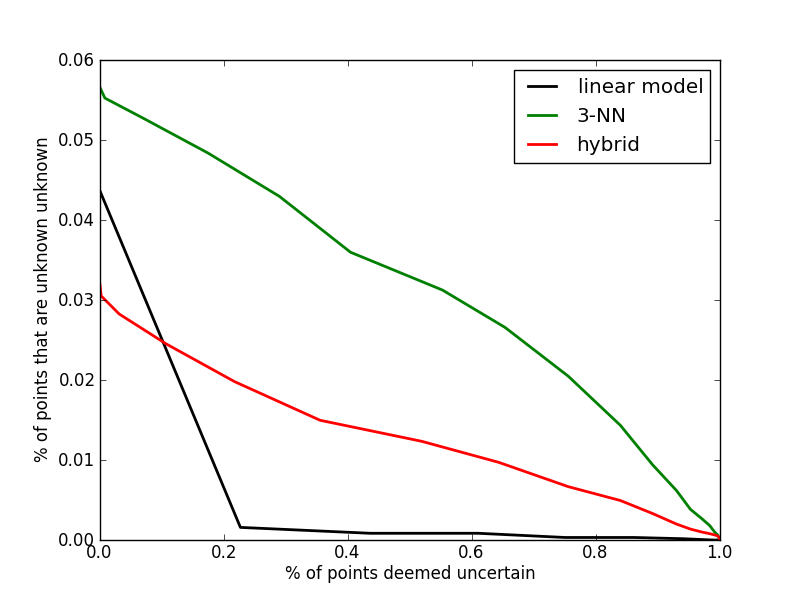
\includegraphics[width= 1.05\columnwidth, height=4.5cm]{plots/decreasing_UU-KU_150_3knn.png}
\label{fig:150}
}
\drop{
\subfigure[$300$ $k$-NN Training Examples]{
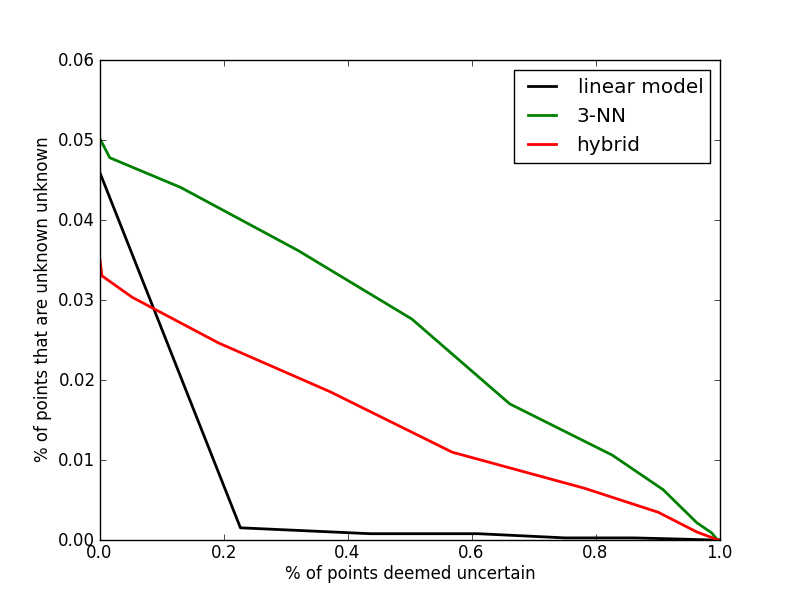
\includegraphics[width= 1.05\columnwidth, height=4.5cm]{plots/decreasing_UU-KU_300_3knn.png}
\label{fig:300}
}
}
\subfigure[$1,500$ $k$-NN Training Examples]{
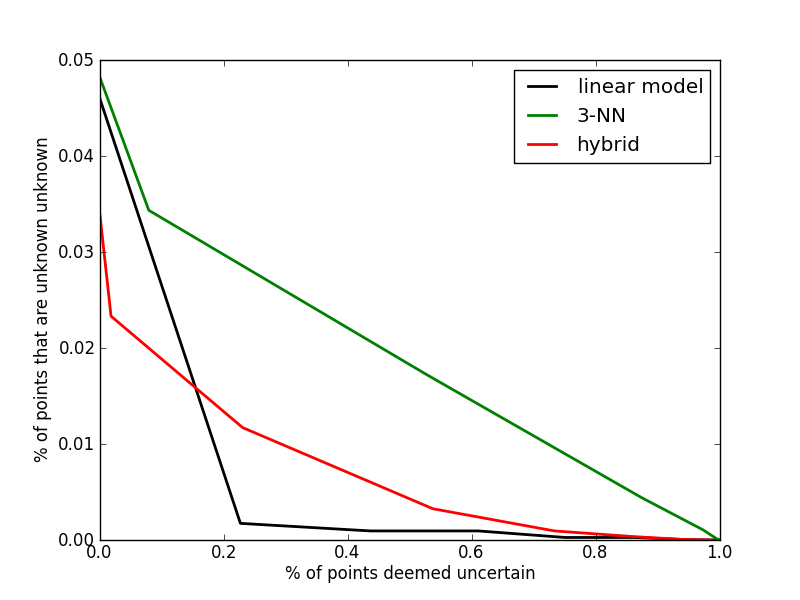
\includegraphics[width= 1.05\columnwidth, height=4.5cm]{plots/decreasing_UU-KU_1500_3knn.png}
\label{fig:1500}
}
\subfigure[$15,000$ $k$-NN Training Examples]{
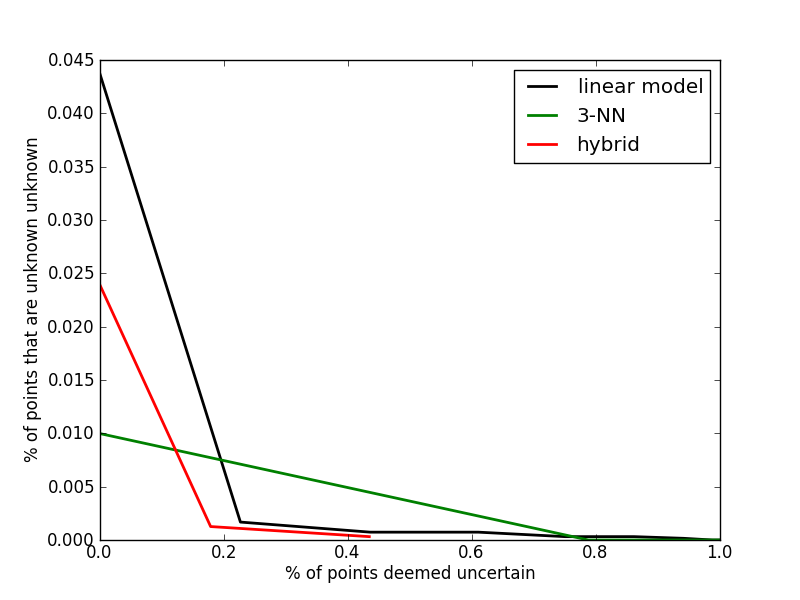
\includegraphics[width= 1.05\columnwidth, height=4.5cm]{plots/decreasing_UU-KU_15000_3knn.png}
\label{fig:15000}
}
}
\caption[caption of subplots]{The tradeoffs between UUs and problem uncertainty for a linear model, KNN, and a hybrid model for differing KNN training sizes}
\label{fig:uuvsku}
\end{figure}

\drop{

\begin{figure}[hbt!]
\begin{center}
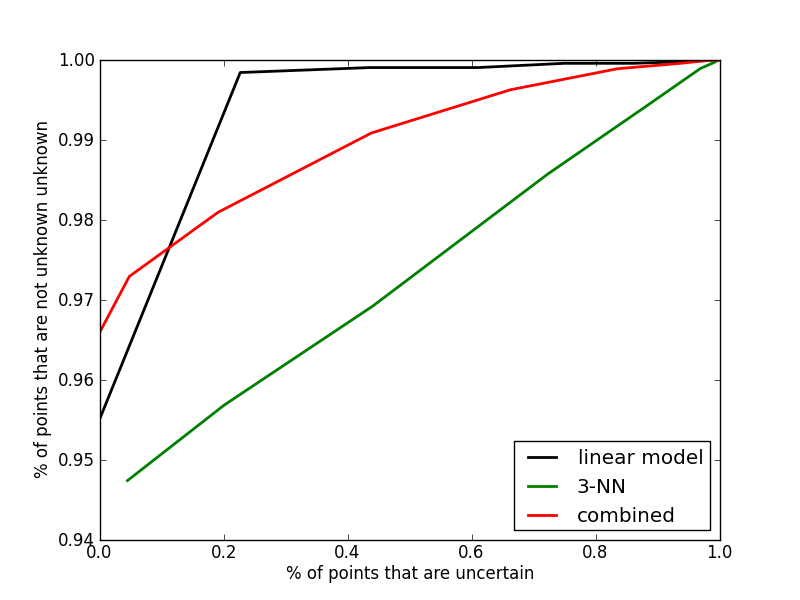
\includegraphics[width= 1.05 \columnwidth]{plots/UU-KU3knn.png}
\end{center}
\vspace{-0.2in}
\caption{The tradeoffs between UUs and problem uncertainty for a linear model, KNN, and a hybrid model }
\label{fig:uuvsku}
\end{figure}
}


